% ======================================================================
%
% Project presentation template in official BUT (Brno University of
% Technology) colors defined by graphical manual in 2015.
%
% Copyright (c) 2018-Present Tomas Fryza, Wykys
% Dept. of Radio Electronics, Brno University of Technology, Czechia
%
% This work is licensed under the terms of the CC BY-NC-SA 4.0 license.
% https://creativecommons.org/licenses/by-nc-sa/4.0/
%
% ======================================================================

\documentclass[aspectratio=1610]{beamer}
\usepackage[english]{babel}
% \usepackage[czech]{babel}
\usepackage[utf8]{inputenc} 
\usepackage{ucs,graphicx,listings,color}

% ----------------------------------------------------------------------

%% COLOR THEME
% \usepackage{themevut} % All in red:)
% \usepackage[FA]{themevut}
% \usepackage[FAST]{themevut}
% \usepackage[FaVU]{themevut}
% \usepackage[FCH]{themevut}
\usepackage[FEKT]{themevut}
% \usepackage[FIT]{themevut}
% \usepackage[FP]{themevut}
% \usepackage[FSI]{themevut}
% \usepackage[CESA]{themevut}
% \usepackage[USI]{themevut}

% ----------------------------------------------------------------------
% TITLE PAGE
% ----------------------------------------------------------------------

% The short title appears at the bottom of every slide, the full title
% is only on the title page.
\title[Short title]
{Full title of the thesis/project/article}

% Type of project, i.e. Semestral, Bachelor, Master's, PhD, etc.
\subtitle
{Semestral/Bachelor/Master's thesis/Conference name}

% Your name
\author[Your NAME]
{
Your NAME\\
% In case of several authors:
% \underline{First AUTHOR}, Second AUTHOR, Third AUTHOR\\
\texttt{email@address}}

% Your institution
\institute
{Department of Radio Electronics\\
Brno University of Technology, Czechia}

% Date, can be changed to a custom date
\date[\today]
{Brno, \today}

% Logo on title page
\titlegraphic{
\includegraphics[height=.15\textheight]{images/logo/logo_fekt_urel.png}}

\begin{document}

% ----------------------------------------------------------------------
% PRESENTATION SLIDES
% ----------------------------------------------------------------------

\begin{frame}
    % Print the title page as the first slide
    \titlepage
\end{frame}


% ----------------------------------------------------------------------
% https://cs.overleaf.com/learn/latex/Lists
\begin{frame}{Lists}
    \textbf{Unordered list}
    \begin{itemize}
        \item Lorem ipsum dolor sit amet, consectetuer adipiscing elit.

        \item Etiam sapien elit, consequat eget, tristique non, venenatis quis, ante.
    \end{itemize}
    \bigskip

    \textbf{Ordered list}
    \begin{enumerate}
        \item \alert{Lorem ipsum dolor} sit amet, consectetuer adipiscing elit.

        \item Aliquam erat volutpat:
        \begin{itemize}
            \item Integer lacinia.

            \item Integer lacinia.
        \end{itemize}
    \end{enumerate}
\end{frame}


% ----------------------------------------------------------------------

\begin{frame}{Multiple columns}
    \begin{columns}
        \column{0.49\textwidth}
        \textit{Lorem ipsum} dolor sit amet, consectetuer adipiscing elit. Etiam sapien elit, consequat eget, tristique non, venenatis quis, ante.
        \bigskip
        
        \texttt{Fusce tellus.} Praesent in mauris eu tortor porttitor accumsan. Nullam feugiat, turpis at pulvinar vulputate, erat libero tristique tellus, nec bibendum odio risus sit amet ante.

        \column{0.49\textwidth}
        \textbf{Lorem ipsum} dolor sit amet, consectetuer adipiscing elit. Etiam sapien elit, consequat eget, tristique non, venenatis quis, ante.
        \bigskip
        
        \underline{Fusce tellus.} Praesent in mauris eu tortor porttitor accumsan. Nullam feugiat, turpis at pulvinar vulputate, erat libero tristique tellus, nec bibendum odio risus sit amet ante.
    \end{columns}
\end{frame}


% ----------------------------------------------------------------------

\begin{frame}{Multiple columns, \textit{cont.}}
    \begin{multicols}{2}
        Lorem ipsum dolor sit amet, consectetuer adipiscing elit. Etiam sapien elit, consequat eget, tristique non, venenatis quis, ante. Duis sapien nunc, commodo et, interdum suscipit, sollicitudin et, dolor.
        \columnbreak
        
        Nullam feugiat, turpis at pulvinar vulputate, erat libero tristique tellus, nec bibendum odio risus sit amet ante. Vestibulum fermentum tortor id mi. Lorem ipsum dolor sit amet, consectetuer adipiscing elit. Etiam sapien elit, consequat eget, tristique non, venenatis quis, ante. Duis sapien nunc, commodo et, interdum suscipit, sollicitudin et, dolor. Fusce tellus. Praesent in mauris eu tortor porttitor accumsan.
    \end{multicols}
\end{frame}


% ----------------------------------------------------------------------

\begin{frame}{Blocks}
    \begin{columns}
        \column{0.3\textwidth}
        \begin{block}{Block}
            Lorem ipsum dolor sit amet, consectetur adipiscing elit. Integer lectus nisl, ultricies in feugiat rutrum, porttitor sit amet augue.
        \end{block}

        \column{0.3\textwidth}
        \begin{exampleblock}{Example block}
            Lorem ipsum dolor sit amet, consectetur adipiscing elit. Integer lectus nisl, ultricies in feugiat rutrum, porttitor sit amet augue.
        \end{exampleblock}

        \column{0.3\textwidth}
        \begin{alertblock}{Alert block}
            Lorem ipsum dolor sit amet, consectetur adipiscing elit. Integer lectus nisl, ultricies in feugiat rutrum, porttitor sit amet augue.
        \end{alertblock}
    \end{columns}
\end{frame}


% ----------------------------------------------------------------------
% https://en.wikibooks.org/wiki/LaTeX/Floats,_Figures_and_Captions
\begin{frame}{Figures}
    \begin{figure}
        \centering
        
\includegraphics[width=0.25\textwidth]{images/logo/logo_symbol.png}
        \caption{Your caption.}
    \end{figure}
\end{frame}


% ----------------------------------------------------------------------
% https://en.wikibooks.org/wiki/LaTeX/Tables
\begin{frame}[fragile]{Tables}
    \lstset{language=[LaTeX]TeX}
\begin{lstlisting}
\begin{table}
    \centering
    \caption{Your caption.}
    \begin{tabular}{l | c | c | r}
        \hline
        \textbf{ID} & \textbf{Duration} & \textbf{Complexity} & \textbf{Score}\\
        \hline
        Algo 1 & 0.0159 & 0.50 & 78\\
        Algo 2 & 0.0453 & 0.65 & 88\\
        Algo 3 & 0.8642 & 0.77 & 95\\
        \hline
    \end{tabular}
\end{table}
\end{lstlisting}
    \begin{table}
        \centering
        \caption{Your caption.}
        \begin{tabular}{l  | c | c |  r}
            \hline
            \textbf{ID} & \textbf{Duration} & \textbf{Complexity} & \textbf{Score}\\
            \hline
            Algo 1 & 0.0159 & 0.50 & 78\\
            Algo 2 & 0.0453 & 0.65 & 88\\
            Algo 3 & 0.8642 & 0.77 & 95\\
            \hline
        \end{tabular}
    \end{table}
\end{frame}


% ----------------------------------------------------------------------
% https://en.wikibooks.org/wiki/LaTeX/Mathematics
\begin{frame}{Equations}
    Pythagorean theorem can be written in one short equation as: $a^2 + b^2 = c^2$ where $c$ is the longest side of the triangle, $a$ and $b$ are the other two sides.

    \vfill % Rubber length which can stretch or shrink vertically

    Other useful equations (thank you \textit{John Napier}):
    \begin{equation}
        \log_b (x^p) = p\cdot \log_b (x)
    \end{equation}

%    \begin{eqnarray*} Start means no numbering
%    \begin{eqnarray}  Equation will have a number
    \begin{eqnarray*}
        \log_b(x) = y & \text{exactly if} & b^y = x
    \end{eqnarray*}
\end{frame}


% ----------------------------------------------------------------------
% https://cs.overleaf.com/learn/latex/Code_listing
\begin{frame}[fragile]{Code listings}
    % Need to use the "fragile" option when verbatim is used in the slide

    \vspace*{-.5cm}
    \begin{columns}
        \column{0.55\textwidth}
\begin{lstlisting}[language=C,title={C example}]
for (uint8_t i = 0; i < LENGTH; i++)
{
    // Test LSB of "segments"
    if ((segments & 0x01) == 0)
        GPIO_write_low(&PORTB, SEGMENT_DATA);
    else
        GPIO_write_high(&PORTB, SEGMENT_DATA);
    // One clock
    SEG_clk_2us();
    // Shift "segments"
    segments = segments >> 1;
}
\end{lstlisting}

        \column{0.43\textwidth}
\begin{lstlisting}[language=Matlab,caption={Matlab example}]
x = 0:0.05:5;
y = sin(x.^2);
figure
% Simple line plot of x and y values
plot(x,y)
\end{lstlisting}
    \end{columns}

\begin{lstlisting}[language=vhdl,title={VHDL example},numbers=left]
---------------------------------------------------------------
-- Entity declaration for hexadecimal to seven-segment decoder
---------------------------------------------------------------
entity hex_7seg is
    port (
        hex : in    std_logic_vector(3 downto 0);
        seg : out   std_logic_vector(6 downto 0)
    );
end entity hex_7seg;
\end{lstlisting}
\end{frame}


% ----------------------------------------------------------------------
% Remind the main results at the end of your presentation
\begin{frame}{Achieved results}
    \begin{itemize}
        \item Lorem ipsum dolor sit amet, consectetuer adipiscing elit.

        \item Etiam sapien elit, consequat eget, tristique non, venenatis quis, ante.

        \item Aliquam erat volutpat.

        \item Integer lacinia.

        \item Cras pede libero, dapibus nec, pretium sit amet, tempor quis.
    \end{itemize}
\end{frame}

% ----------------------------------------------------------------------
% It is a common practice you already have reviewer(s) comments/questions before your presentation. Sometimes, it is useful to prepare extra slides to answer those questions.
\begin{frame}{Reviewer's questions}
    \begin{exampleblock}{Question 1}
        Lorem ipsum dolor sit amet, consectetur adipiscing elit?
    \end{exampleblock}
    \bigskip

    \begin{block}{Answer 1}
        Lorem ipsum dolor sit amet, consectetur adipiscing elit. Integer lectus nisl, ultricies in feugiat rutrum, porttitor sit amet augue. Aliquam ut tortor mauris. Sed volutpat ante purus, quis accumsan dolor.
    \end{block}
\end{frame}

% ----------------------------------------------------------------------

\begin{frame}{Q \& A}
    \begin{columns}
        \column{0.5\textwidth}
        \begin{flushright}
            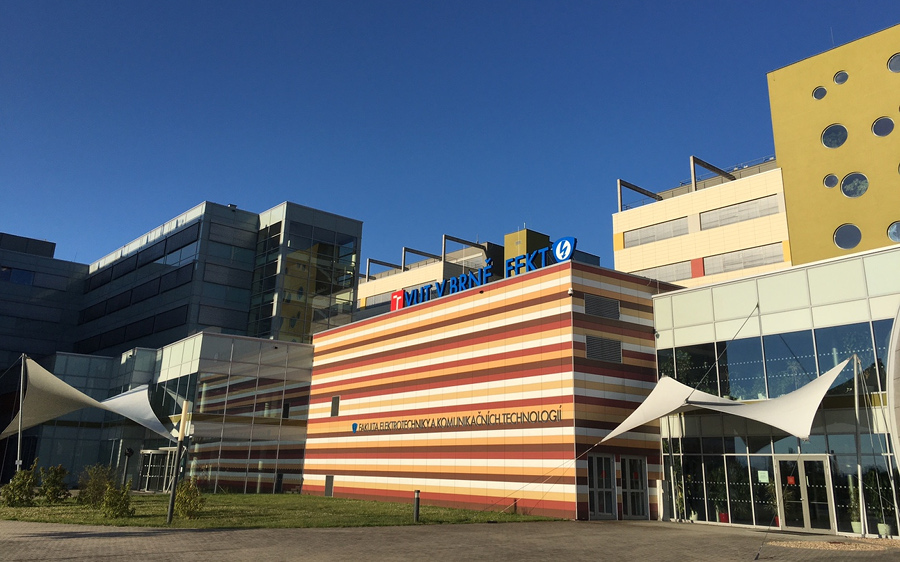
\includegraphics[width=1.\textwidth]{images/contacts/fekt_leto.jpg}
        \end{flushright}

        \column{0.5\textwidth}
        \textbf{Your NAME}\\
        ~\\
        Department of Radio Electronics\\
        Brno University of Technology\\
        % \url{https://www.vutbr.cz/lide/tomas-fryza-11389}\\
        \url{https://www.urel.fekt.vut.cz}\\
        ~\\
        \url{fryza@vut.cz}\\
        ~\\
        
\includegraphics[scale=0.5]{images/contacts/icon_fcb.png} \url{https://www.facebook.com/URELBrno}\\

        
\includegraphics[scale=0.5]{images/contacts/icon_github.png} \url{https://www.github.com/your-acount}\\

        
\includegraphics[scale=0.5]{images/contacts/icon_twitter.png} @YourName\\
    \end{columns}
% -------------------------------------
    \note{~}
% -------------------------------------
\end{frame}

\end{document}
